\documentclass[11pt]{article}
\usepackage[a4paper,margin=2cm]{geometry}
\usepackage[brazilian]{babel}
\usepackage[utf8]{inputenc}
\usepackage[T1]{fontenc}
\linespread{1.3}
\parskip=12pt
\parindent=0pt
\usepackage{enumitem}
\usepackage{amsmath}
\usepackage{amsfonts}
\usepackage{graphicx}
\usepackage{amssymb}
\usepackage{hyperref}
\usepackage{amsthm}
\usepackage{color}


% Defining the question styles
\theoremstyle{definition}
\newtheorem{prob}{Problem}

\theoremstyle{definition}
\newtheorem{problema}{Problema}

% Custom commands
\newcommand{\E}{\mathbb{E}}
\newcommand{\Var}{\mathrm{Var}}
\newcommand{\Prob}{\mathbb{P}}

% declare a new theorem style
\newtheoremstyle{solution}%
{1pt}% Space above
{1pt}% Space below 
{\itshape\color{red}}% Body font
{}% Indent amount
{\bfseries\color{red}}% Theorem head font
{.}% Punctuation after theorem head
{.5em}% Space after theorem head
{}% Theorem head spec (can be left empty, meaning ‘normal’)

\theoremstyle{solution}
\newtheorem*{solution}{Solution}

% --- Code starts here ---
\begin{document}
	\begin{center}
		{\Large{\textbf{Lista II - Métodos Numéricos}}}\\
		\vspace{0.2cm}
		EPGE - 2018\\
		Professor: Cézar Santos\\
		Aluno: Raul Guarini Riva
	\end{center}

\begin{problema}
	O problema no planejador consiste em escolher recursivamente quanto consumir no presente e quanto poupar na forma de capital para o próximo período, tendo por base o estado da economia formado pelo estoque de capital atual e a produtividade atual. 
	
	A função utilidade das famílias não leva em consideração o lazer. Desta forma, ofertarão trabalho inelasticamente. Normalizando a dotação de trabalho para uma unidade, a equação funcional com a qual o planejador se defronta é a seguinte:
	\begin{gather*}
		V(K, z) = \max\limits_{c, K'} \{u(c) + \beta\E[V(K', z')|z] \} \\
		\text{s.t.} \quad c + K' \leq zK^{\alpha} + (1-\delta)K
	\end{gather*}
	
	A hipótese de $u$ estritamente crescente implica que a restrição de recursos será satisfeita com igualdade em todo instante do tempo. Daí, reescreve-se:
	\begin{gather*}
		V(K,z) = \max\limits_{K'}\{u(zK^{\alpha} + (1-\delta)K - K') + \beta\E[V(K', z')|z]\}
	\end{gather*}
\end{problema}

\begin{problema}
	Supondo não haver incerteza, normaliza-se o valor da produtividade para a média incondicional do processo:
	\begin{equation*}
		\log(z) = 0 \implies z = 1
	\end{equation*}
	
	A equação de Euler é dada por
	\begin{gather*}
		\beta\E\bigg[\left(\frac{c'}{c}\right)^{-\mu}(z'\alpha K'^{\alpha - 1} + 1 - \delta)\big|z\bigg] = 1
	\end{gather*}
	Sem incerteza e já resolvendo para o estado estacionário:
	\begin{gather*}
		\beta\alpha K^{\alpha -1}_{ss} = 1 - \beta(1-\delta)\\
		\boxed{K_{ss} = \left(\frac{\alpha\beta}{1 - \beta(1-\delta)} \right)^{\frac{1}{1-\alpha}}}
	\end{gather*}
	
	Com a calibração sugerida na lista, temos $K_{ss} = 48.1905$.
\end{problema}

\begin{problema}
	Para esta primeira implementação, explorei a monotonicidade da função política e a concavidade do funcional sendo otimizado. O código está no formato de uma função chamada \texttt{VFinder\_Iterated.m}, devidamente documentada através do próprio \texttt{help} do MATLAB.
	
	A primeira iteração foi feita através de força bruta e as próximas seguiram explorando os aspectos teóricos do problema. Abaixo, a função valor e a função política (como esperado, crescente!!!):
	\begin{figure}[htb!]
		\centering
		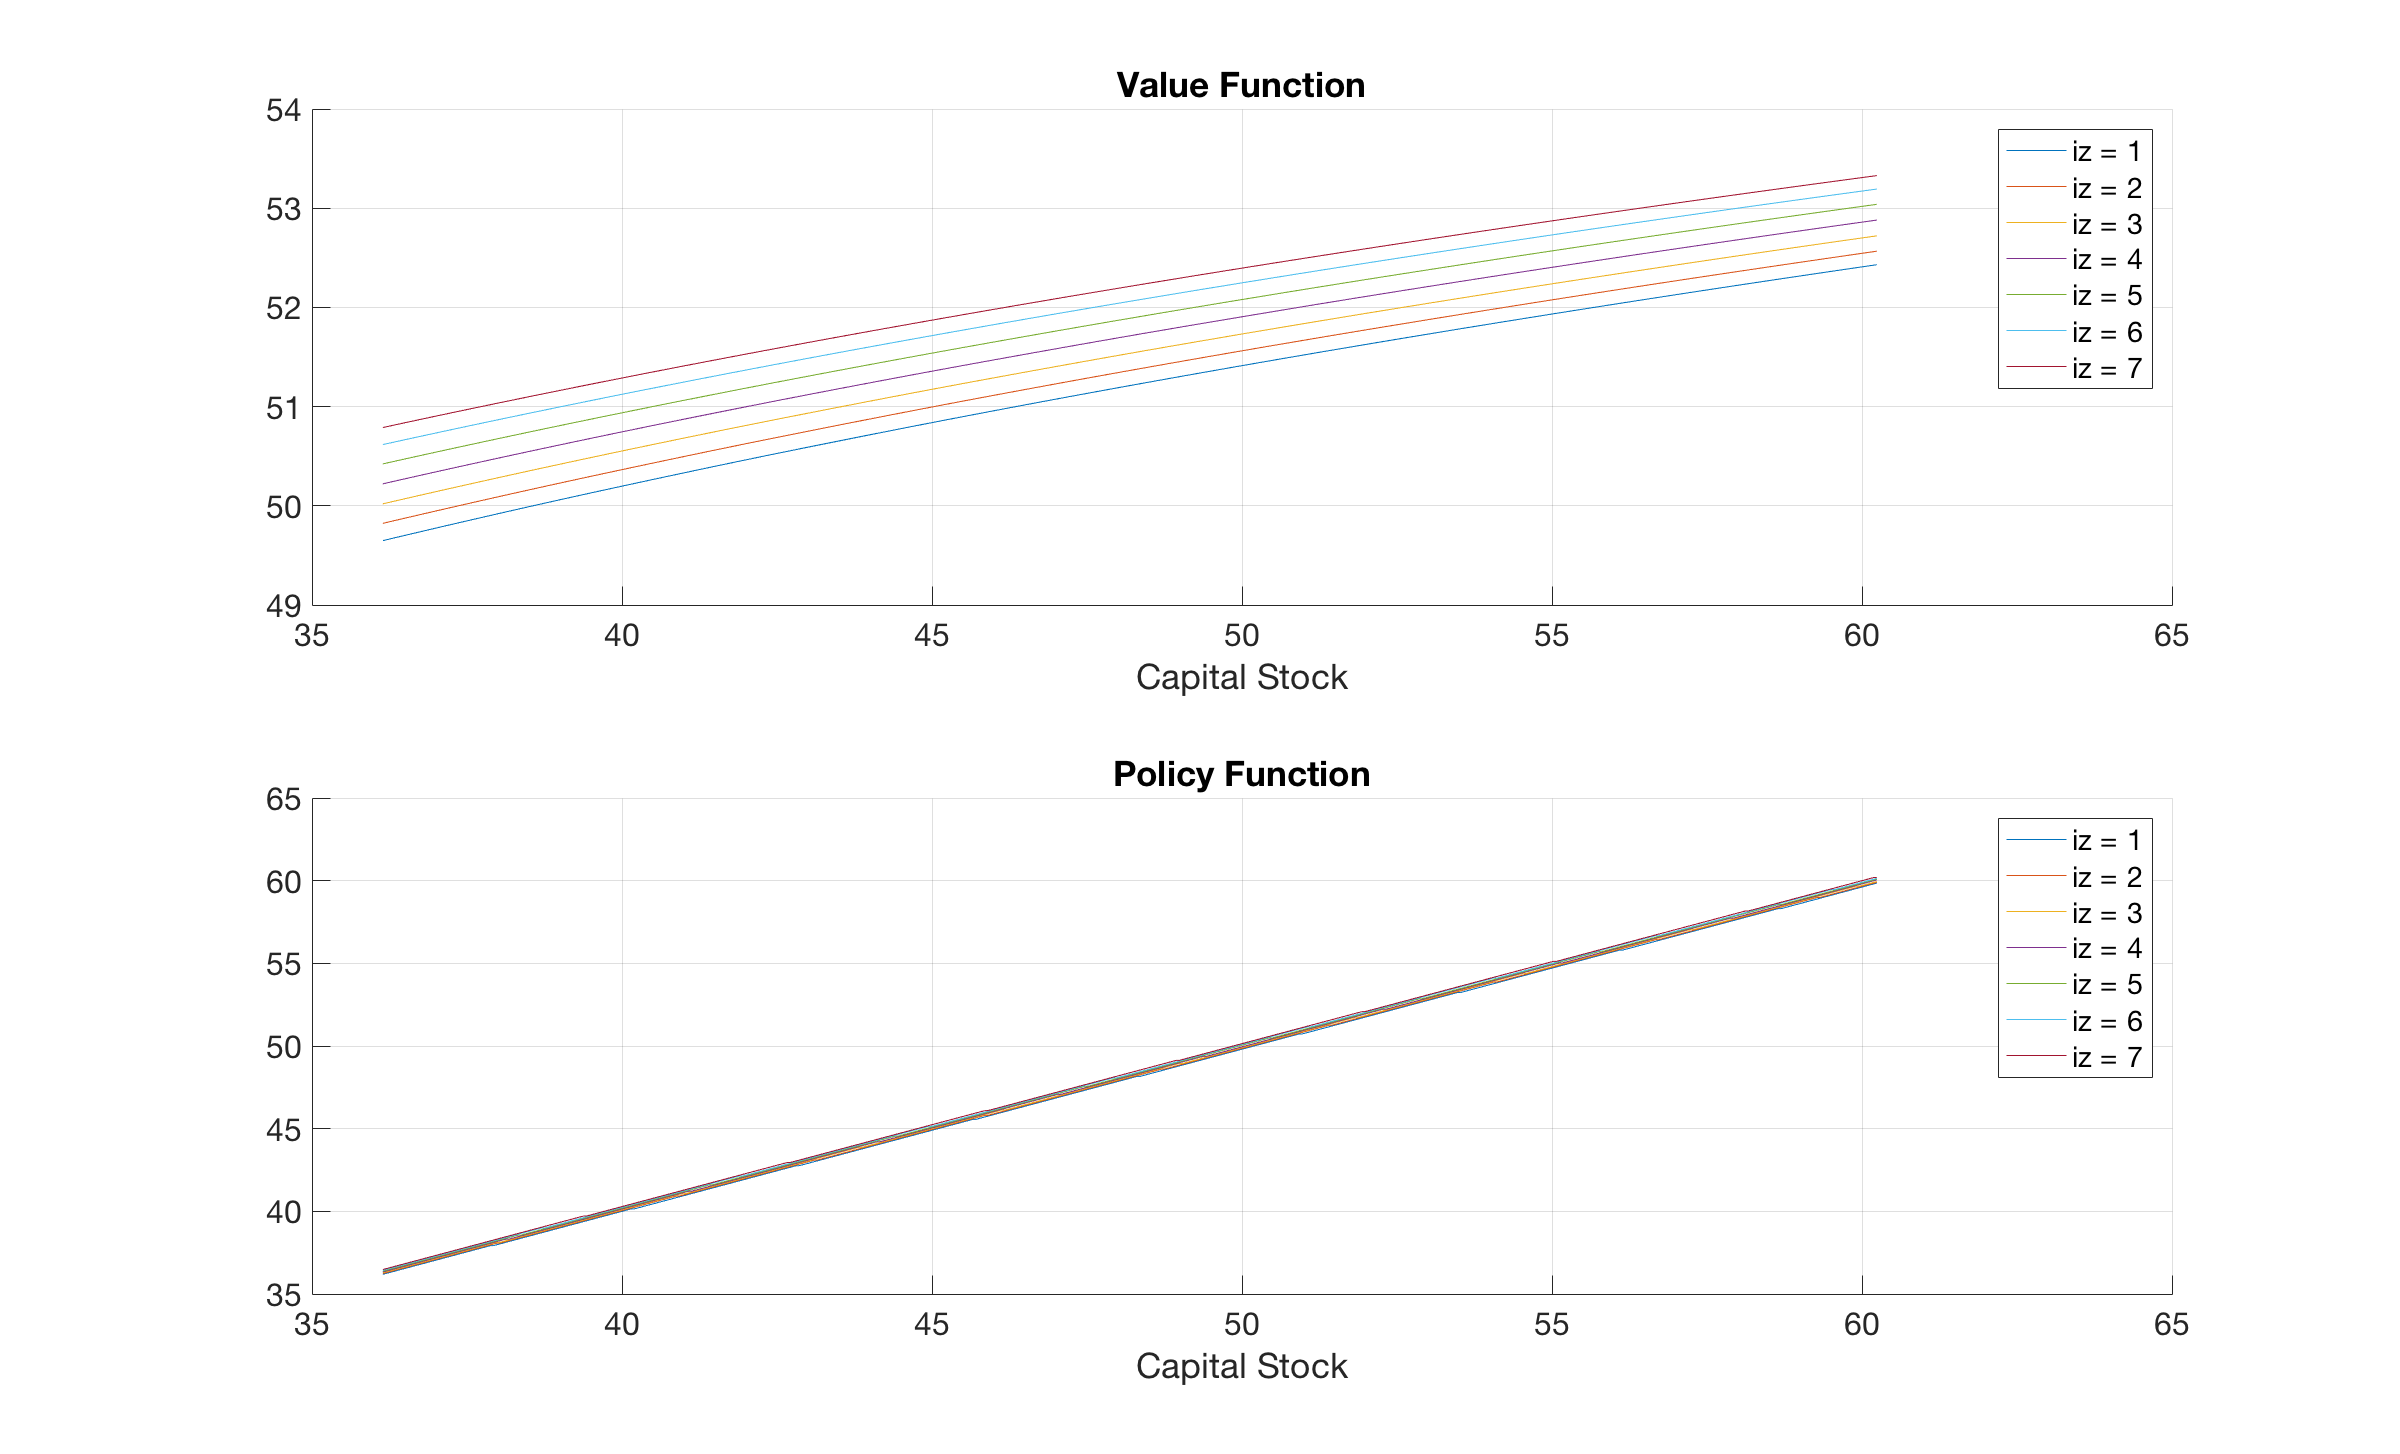
\includegraphics[scale = 0.22]{problem3_V_vs_G}
	\end{figure}
	
	Obtive o resultado, também esperado, de que a função valor, para um valor de $k$ fixo, é crescente na TFP. A legenda iz $= 4$, por exemplo, indica que determinada curva foi computada com o valor da TFP correspondente ao quarto ponto do grid do choque $\log (z)$.
	
	Para comparar o desempenho desta abordagem (que não utiliza nenhum tipo de vetorização), implementei o método de ``força bruta vetorizada''. Isto é, operar maximizações ao longo das dimensões de arrays do MATLAB evitando criar ``for loops''. Esta abordagem está no script \texttt{brute\_force.m}.
	
	Houve um ganho de desempenho considerável. O método de força bruta vetorizada computou a função valor e a função política em 8.85 segundos. O método que utiliza a função \texttt{VFinder\_Iterated.m} resolveu o mesmo problema em 6.39 segundos. Isto representa um ganho de quase 28\%, o que considero expressivo. 
	
	Nota-se, entretanto, que o método de força bruta é mais geral que seu concorrente, em vista do fato que funcionaria igualmente bem para um problema em que não tivéssemos um resultado teórico garantindo a monotonicidade da função política ou a concavidade do funcional em questão. Uma performance pior é o preço a ser pago pela maior versatilidade.

	
	\end{problema}
\end{document}
